\documentclass{article}
\usepackage{xcolor}
\usepackage{tikz-cd}
\usepackage{amsmath}
\usepackage{amssymb}
\usepackage{amsthm}
\usepackage{enumitem}
\usepackage{mathtools}
\usepackage{graphicx}
\usepackage{wrapfig}
\usepackage[a4paper, total={6in, 8in}]{geometry}
\usepackage{pgfplots}
\pgfplotsset{compat=1.15}
\usepackage{mathrsfs}
\usetikzlibrary{arrows}

% environments
\theoremstyle{definition}
\newtheorem*{definition}{Definition}
\newtheorem*{example}{Example}
\newtheorem{exercise}{Exercise}

\theoremstyle{plain}
\newtheorem{theorem}{Theorem}
\newtheorem{corollary}[theorem]{Corollary}
\newtheorem{proposition}{Proposition}
\newtheorem{lemma}{Lemma}

\theoremstyle{remark}
\newtheorem*{remark}{Remark}
\newtheorem*{fact}{Fact}

\newenvironment{claim}[1]{\par\underline{Claim:}\space#1}{\par\smallskip}
\newenvironment{acase}[1]{\par\underline{Case\space#1:}\space}{\par\smallskip}
\newcommand{\astep}[2]{\par\textbf{Step #1: #2}\par\smallskip}

\numberwithin{equation}{section}
% commands
\newcommand{\contra}{\Rightarrow\!\Leftarrow}

\newcommand{\bZ}{\mathbb{Z}}
\newcommand{\bQ}{\mathbb{Q}}
\newcommand{\bR}{\mathbb{R}}
\newcommand{\bC}{\mathbb{C}}

\newcommand{\rangewith}[4]{{#2}#1{#3}, \cdots, {#2}#1{#4}}
\newcommand{\funtyp}[3]{#1: & #2 & \rightarrow & #3 \\ }
\newcommand{\fundecl}[2]{& #1 & \mapsto & #2 \\ }

\newcommand{\abs}[1]{\left| {#1} \right|}
\newcommand{\inprod}[2]{\langle {#1}, {#2} \rangle}

\newcommand{\im}{{\sqrt{-1}}}

\DeclareMathOperator{\sgn}{sgn}

\def\ns{{\mathbf{n}}}
\def\nsL{{\mathbf{n}_L}}
\def\nsR{{\mathbf{n}_R}}

% GeoGebra
\definecolor{geoblue}{rgb}{0.08235294117647059,0.396078431372549,0.7529411764705882}
\definecolor{geored}{rgb}{0.8274509803921568,0.1843137254901961,0.1843137254901961}

\title{Sketch of $u$-degree finder algorithm on $\bC$}
\author{Junho Lee}

\begin{document}
\maketitle

Fix $\lambda \in \bC$, and denote
\[
  \ns = (\nsL, n_i, \nsR) = (\nsL', n_{i-1}, n_i, n_{i+1}, \nsR').
\]
sequences of $\bar{\bZ} \setminus \{0\}$.
We assume length of $\ns$ is no more than the minimal $u$-degree of $\lambda$.
We are interested with computing
\[
  M_k := \max_{\ns \in (\bar{\bZ} \setminus \{0\})^k} \abs{[\ns]},
\]
which should exist by compactness of $\bar{\bZ} \setminus \{0\}$.
As an intermediate step, we will compute
\[ M^{\nsL} := \max_{n_i, \nsR} \abs{[\nsL, n_i, \nsR]}. \]
where $M_k$ falls out from $M_k = M^{()}$.

Recall that for $i \geq 2$,
\begin{align*}
  [\ns] & = [\nsL] \cdot \frac{n_i + [\overleftarrow{\nsL}'] + [\nsR]}{n_i + [\overleftarrow{\nsL}] + [\nsR]} \\
  & = [\nsL] \left( 1 - \frac{[\overleftarrow{\nsL}] - [\overleftarrow{\nsL}']}{n_i + [\nsL] + [\nsR]} \right).
\end{align*}

Denote the singular point as $N_i = - ([\overleftarrow{\nsL}] + [\nsR])$,
and define \textit{discriminant} $D := [\overleftarrow{\nsL}] - [\overleftarrow{\nsL}']$ to write
\[
  [\ns] = [\nsL] \left( 1 - \frac{D}{n_i - N_i} \right).
\]
For fixed $\nsL$,
\[
  M^{\nsL} = \max_{n_i, \nsR} \abs{[\ns]} = \abs{[\nsL] D} \cdot \max_{n_i, \nsR} \left| \frac{1}{D} - \frac{1}{n_i - N_i} \right|.
\]

Meanwhile, if $i = 1$, $[\ns] = \frac{1 / \lambda}{n_i + [\nsR]}$.
Hence, we may take $N_i = - [\nsR]$ and $D = \infty$ so that
\[
  M^{()} = \frac{1}{\abs{\lambda}} \max_{n_i, \nsR} \abs{\frac{1}{\infty} - \frac{1}{n_i - N_i}}.
\]

First, we estimate $n_i$ in the maximal case by trying different values in its place.

\begin{lemma}\label{maximal case estimate}
  Suppose $\frac{D}{2 \Im(N_i) \im} \neq 0, -1$.
  Then, $(x \mapsto \abs{[\nsL, x, \nsR]}) : \bar{\bR} \to [0, \infty]$ has a unique local maximum at $x = x_{\max}$, given as
  \begin{equation*}
    x_{\max} - a = \begin{dcases}
      - \frac{\abs{D} \abs{D + 2b \im} - \inprod{D}{D + 2b \im}}{2 \Re(D)}, & \Re(D) \neq 0 \\
      \infty, & D / (2b \im) \in (-1, 0) \\
      0, & D / (2b \im) \in \bar{\bR} \setminus (-1, 0)
    \end{dcases}
  \end{equation*}
  where $N_i = a + b \im$, $a, b \in \bR$
  and $\inprod{-}{-}$ is a $\bR$-bilinear form given by $\inprod{c + d \im}{c' + d' \im} = cc' + dd'$.
\end{lemma}
\begin{proof}
  Consider that the M\"{o}bius transformation $\varphi(z) = z^{-1}$ sends $\bR - N_i$ to a line or a circle.
  When it is mapped to a line, it passes through the origin,
  so $x_{\max} = N_i \in \bR$ obtains the maximum $\infty$; one can check this matches the desired conclusion.
  Hence, enough to check the general case where $\varphi(\bR - N_i)$ is a circle passing through origin.

  \begin{center}
    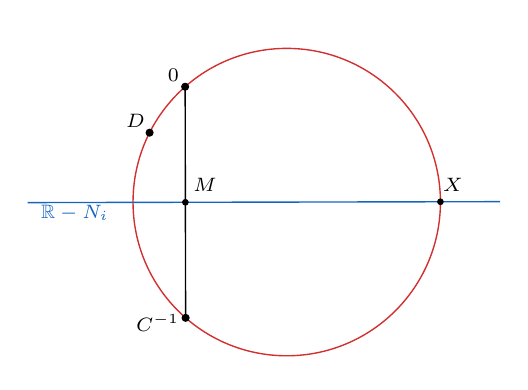
\begin{tikzpicture}[line cap=round,line join=round,>=triangle 45,scale=0.5]
      \clip(-9,-4) rectangle (3,4.5);
      \draw [line width=0.5pt,color=geored] (-2.42,0.07) circle (3.9040107581818986cm);
      \draw [line width=0.5pt] (-5,3)-- (-4.988339894200145,-2.8702262137223373);
      \draw [line width=0.5pt,color=geoblue,domain=-9:3] plot(\x,{(--0.43913329099621135--0.011660105799855103*\x)/5.870226213722337});
      \begin{scriptsize}
        \draw [fill=black] (-5,3) circle (2.5pt);
        \draw[color=black] (-5.3,3.3) node {$0$};
        \draw [fill=black] (-4.988339894200145,-2.8702262137223373) circle (2.5pt);
        \draw[color=black] (-5.7,-3) node {$C^{-1}$};
        \draw[color=geoblue] (-7.8,-0.2) node {$\bR-N_i$};
        \draw [fill=black] (-4.9941699471000724,0.06488689313883132) circle (2pt);
        \draw[color=black] (-4.5,0.5) node {$M$};
        \draw [fill=black] (1.4840030566869966,0.07775457146396089) circle (2pt);
        \draw[color=black] (1.8,0.5) node {$X$};
        \draw [fill=black] (-5.903419240287578,1.8326940733985344) circle (2.5pt);
        \draw[color=black] (-6.26,2.14) node {$D$};
      \end{scriptsize}
    \end{tikzpicture}
    \hspace{0.5cm}
    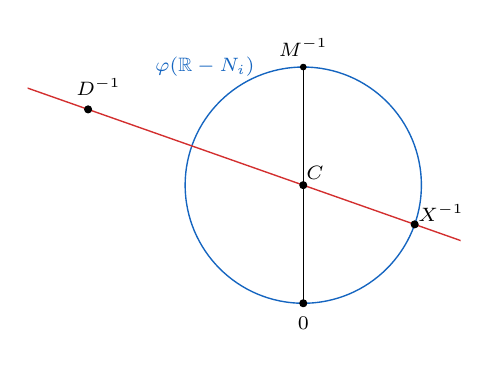
\begin{tikzpicture}[line cap=round,line join=round,>=triangle 45,scale=0.5]
      \clip(1,-3) rectangle (12,5);
      \draw [line width=0.5pt,color=geoblue] (8,1) circle (3cm);
      \draw [line width=0.5pt,color=geored,domain=-4.54:21.06] plot(\x,{(-10.800708883665594--0.9963753582717338*\x)/-2.8297060174917235});
      \draw [line width=0.5pt] (8,4)-- (8,-2);
      \begin{scriptsize}
        \draw [fill=black] (8,1) circle (2.5pt);
        \draw[color=black] (8.3,1.3) node {$C$};
        \draw [fill=black] (8,-2) circle (2.5pt);
        \draw[color=black] (8,-2.5) node {$0$};
        \draw[color=geoblue] (5.5,4) node {$\varphi(\bR-N_i)$};
        \draw [fill=black] (10.829706017491723,0.0036246417282661536) circle (2.5pt);
        \draw[color=black] (11.5,0.3) node {$X^{-1}$};
        \draw [fill=black] (8,4) circle (2pt);
        \draw[color=black] (8,4.5) node {$M^{-1}$};
        \draw [fill=black] (2.5345287680903645,2.9244617013766323) circle (2.5pt);
        \draw[color=black] (2.8,3.5) node {$D^{-1}$};
      \end{scriptsize}
    \end{tikzpicture}
  \end{center}

  Note we can identify the circle's center $C \in \bC$ as follows.
  Let $M = - \Im(N_i) \im$, an intersection of the imaginary line $\im \bR$ and $\bR - N_i$.
  $\varphi$ sends $M$ to an intersection of the imaginary line and $\varphi(\bR - N_i)$,
  where the two meets orthogonally.
  Hence, $C$ is the midpoint of $M^{-1}$ and $0$, i.e. $C = M^{-1}/2$,
  and so $C^{-1} = 2M = - 2 \Im(N_i) \im$.

  Now, observe that
  \[
    \abs{[\nsL, x, \nsR]} = \abs{D^{-1} - (x - N_i)^{-1}}
  \]
  is the distance from $(x - N_i)^{-1} \in \varphi(\bR - N_i)$ to $D^{-1}$.
  Clearly it has a unique local maximum,
  which is obtained when the center $C$ lies on the line segment from $D^{-1}$ to $(x - N_i)^{-1}$.
  Remark that this works just as well for $D = \infty$ as $D^{-1} = 0 \neq C$.
  Say, the local maximum occurs at $x = x_{\max}$, and let $X = x_{\max} - N_i$.
  Then $X^{-1}, C, D^{-1}$ are colinear in this order.
  Hence, the cross ratio is given by
  \[
    (\infty, C; D^{-1}, X^{-1}) = \frac{X^{-1} - C}{D^{-1} - C} = \gamma_X \in \bR_{< 0}
  \]
  and taking $\varphi^{-1}$,
  \[
    \gamma_X = (0, C^{-1}; D, X) = \frac{D - 0}{D - C^{-1}} \cdot \frac{X - C^{-1}}{X}.
  \]
  As $\abs{X - C^{-1}} = \abs{X}$,
  we get $\gamma_X = - \frac{\abs{D}}{\abs{D - C^{-1}}}$ from the absolute value. Thus,
  \[
    e^{\im \theta} := \frac{X - C^{-1}}{X}
    = - \frac{(D - C^{-1}) / D}{\abs{D - C^{-1}} / \abs{D}}
    = - \frac{\bar{D} (D - C^{-1})}{\abs{D} \abs{D - C^{-1}}}.
  \]
  Notice that $\Re(\bar{D} (D - C^{-1})) = \inprod{D}{D - C^{-1}}$.
  Using this, one can check $\cos \theta = - \frac{\inprod{D}{D - C^{-1}}}{\abs{D} \abs{D - C^{-1}}}$
  and $\sin \theta = \frac{\Re(D) \Im(C^{-1})}{\abs{D} \abs{D - C^{-1}}}$.
  Also, from $M = C^{-1} / 2$ one has
  $\frac{X - M}{M} = \frac{1 + e^{\im \theta}}{1 - e^{\im \theta}}$.

  Note that if $D < \infty$ and $\Re(D) \neq 0$, $\sin \theta \neq 0$, so we get
  \[
    X - M = M \frac{1 + \cos \theta}{\sin \theta} = - \frac{|D| |D - C^{-1}| - \inprod{D}{D - C^{-1}}}{2 \Re(D)} \in \bR.
  \]
  On the other hand, if $\Re(D) = 0$,
  one has $e^{\im \theta} = - \sgn(\Im(D) (\Im(D) - \Im(C^{-1}))) = \pm 1$;
  thus $X - M = 0$ or $\infty$ depending on values of $\Im(D)$ and $\Im(C^{-1})$.
  Also, similar holds for $D = \infty$ as well.
  In both cases, the conclusion follows by taking the real part of the equation.
\end{proof}

\begin{remark}
  $\abs{[\nsL, x, \nsR]}$ is constant if the discriminant is $D = 0$ or $D = - 2 \Im(N_i) \im$.
  Indeed, $[\nsL, x, \nsR] = [\nsL]$ if $D = 0$,
  and the center $C$ coincides with $D^{-1}$ if $D = -2 \Im(N_i) \im$.
  In these cases, one can say that $\abs{[\nsL, x, \nsR]}$ is 'maximal' for every $x \in \bar{\bR}$.

  In fact, $D = 0$ case does not occur unless $\nsL$ contains infinity;
  the recurrence relation takes
  $[n_{i-1}, n_{i-2}, \cdots, n_1] = [n_{i-1}, n_{i-2}, \cdots, n_2]$
  into $n_{i-1} + [n_{i-2}, \cdots, n_1] = n_{i-1} + [n_{i-2}, \cdots, n_2]$,
  where $n_{i-1}$ can be cancelled out in absence of infinity.
  This descent ends at $[n_1] = []$, and this yields contradiction.
\end{remark}

% TODO Consider generalizing so that infinity case is streamlined
\begin{proposition}\label{maximal ni estimate}
  The maximum $M^{\nsL}$ can be obtained from $\ns = (\nsL, n_i, \nsR)$ satisfying
  \[
    \begin{cases}
      \abs{n_i - \left(\Re(N_i) - \frac{\delta(2 \Im(N_i))}{2 \Re(D)} \right)} < 2, & \Re(D) \neq 0, \\
      \abs{n_i - \Re(N_i)} < 2 \text{ or } n_i = \infty, & \Re(D) = 0
    \end{cases}
  \]
  where $\delta(t) = \abs{D} \abs{D + t \im} - \inprod{D}{D + t \im}$.
\end{proposition}
\begin{proof}
  First, we show the case of $\Re(D) \neq 0$.
  Consider the particular $\ns = (\nsL, n_i, \nsR)$ which attains the maximum.
  Then, clearly
  \[ M^{\nsL} = \max_{n_i, \nsR} [\nsL, n_i, \nsR] = \max_{n_i \in \bar{\bZ} \setminus \{0\}} [\nsL, n_i, \nsR]. \]

  Let $f(x) = \abs{[\nsL, x, \nsR]}$ which is a continuous function on $\bar{\bR} \cong S^1$.
  By Lemma \ref{maximal case estimate}, $f$ only has one local maximum $x_{\max} < \infty$.
  Notice that there are $l, r \in \bZ \setminus \{0\}$
  such that $l \leq x_{\max} \leq r$ and interval $(l, r)$ does not contain any nonzero integer.
  Now,
  \[
    M^{\nsL} = \max_{n_i \in \bar{\bZ} \setminus \{0\}} f(n_i) = \max(f(l), f(r))
  \]
  since $f$ cannot be larger than $\max(f(l), f(r))$ outside $[l, r]$, considering absence of local maximum outside the range.
  By replacing $n_i$ with $l$ or $r$ if necessary, one has the desired consequence of $\abs{n_i - x_{\max}} < 2$.

  On the other hand, if $\Re(D) = 0$ the local maximum, we have 3 cases:
  either $x_{\max} - \Re(N_i) = 0$ or $\infty$, or $f$ might be constant over $\bar{\bR}$.
  Once $x_{\max} = \Re(N_i)$ which is finite, we get $\abs{n_i - \Re(N_i)} < 2$ as above.
  Otherwise, $x_{\max} = \infty$ or $f$ is constant so
  \[
    M^{\nsL} = \max_{n_i \in \bar{\bZ} \setminus \{0\}} f(n_i) = f(\infty),
  \]
  and $n_i$ may be replaced with $\infty$.
  To sum up, we may take $n_i$ with $\abs{n_i - \Re(N_i)} < 2$ or $n_i = \infty$ if $\Re(D) = 0$.
\end{proof}

The following behavior of $\delta(t)$ will be used to compute
the appropriate bounds of $\Re(N_i) - \frac{\delta(2 \Im(N_i))}{2 \Re(D)}$ over varying $\nsR$.

\begin{lemma}
  $\delta(t)$ only has a local minimum at $t = 0$, and it has no local maximum.
  Hence, $0 \leq \delta(t) \leq \max(\delta(a), \delta(b))$ whenever $t \in [a, b]$.
\end{lemma}
\begin{proof}
  By differentiating, one has
  \[
    \delta'(t) = \abs{D} \left( \frac{\inprod{D + ti}{i}}{\abs{D + ti}} - \frac{\inprod{D}{i}}{\abs{D}} \right)
  \]
  which is an increasing function in $t$ by the behavior of projection. Also, $\delta'(0) = 0$.
\end{proof}

Now, we are ready to compute the maximum $M^{\nsL} = \max_{n_i, \nsR} \abs{[\nsL, n_i, \nsR]}$,
whose process is outlined below.
\begin{enumerate}
  \item Compute $D$, and compute range of $N_i$ (denoted $\mathcal{B} \subset \bC$)
        using $\abs{N_i + [\overleftarrow{\nsL}]} \leq \max \abs{[\nsR]} = M_{k-i}$.
  \item Compute range $\mathcal{N} \subset \bar{\bZ} \setminus \{0\}$ of $n_i$ depending on $D$.
  \begin{enumerate}
    \item If $\Re(D) = 0$, $\abs{n_i - \Re(N_i)} < 2$ or $n_i = \infty$,
          so $\mathcal{N} = (\Re(\mathcal{B}) + (-2, 2)) \cup \{\infty\}$.
    \item If $\Re(D) \neq 0$, compute $\Delta = \max_{t \in 2 \partial \Im(\mathcal{B})} \delta(t)$.
          Then, $\delta(2 \Im(N_i)) \in [0, \Delta]$, so together with Proposition \ref{maximal ni estimate} one has
          \[ \mathcal{N} = \Re(\mathcal{B}) - \frac{1}{2 \Re(D)} \cdot [0, \Delta] + (-2, 2). \]
  \end{enumerate}
  \item Compute $M^{\nsL} = \max_{n_i \in \mathcal{N}} M^{(\nsL, n_i)}$ recursively.
        Remark that for $n_i = \infty$,
        $M^{(\nsL, n_i)}$ is trivial to compute since $[\nsL, \infty, \nsR] = [\nsL]$ always holds.
\end{enumerate}

In the process, we obtain the maximum over all $\ns$ as $M_k = M^{()}$.
Furthermore, $k$ is the minimal $u$-degree once we obain $M_k = \infty$.
Therefore, this gives an algorithm for finding the minimal $u$-degree.

\begin{remark}
  If $\lambda \in \bR$, one has both $N_i \in \bR$ and $D \in \bR$.
  By inductive argument,
  one can see that $D \neq 0$ and $\abs{n_i - N_i} < 2$ for each $i$ in the maximal case.
  This gives a simpler bound of $\abs{n_i + [\overleftarrow{\nsL}]} < M_{k-i} + 2$,
  and $M_k > M_{k-i}$.
\end{remark}

\end{document}